\section{PandoraPFA}

\subsection{Collaborating Institutions}

Development of the Pandora framework and algorithms has been based exclusively
in Cambridge, but detector optimisation studies have involved close
collaboration with other institutes. ECAL and analogue HCAL studies have
involved DESY, Shinsu University (Japan), and CERN. Upcoming (semi-)digital HCAL
studies will involve the University of Lyon (France).

\subsection{Introduction}
\subsection{Recent Milestones}
The PandoraPFA software package~\cite{Thomson200925,Marshall2013153}
has been developed entirely in Cambridge.
It consists of a robust and efficient C++ software development kit (SDK) and
libraries of reusable pattern-recognition algorithms that exploit functionality
provided by the SDK. Algorithms have been developed to provide a particle flow
reconstruction of events in fine-granularity detectors, such as those proposed
for use at the ILC or CLIC. The reconstruction uses over 60 algorithms in order
to carefully trace the paths of visible particles through the detector. The
output is a complete list of the particles in an event, each with a
reconstructed four-momentum and an identified particle-type. The algorithms
represent the state-of-the-art in particle flow calorimetry at a Linear
Collider. The Pandora Linear Collider algorithms have recently been used for
extensive detector optimisation studies, assessing the physics performance of
the ILD\_o1\_v06 detector model with different configurations of the
electromagnetic and hadronic calorimeters. A selection of the key plots is shown
overleaf. A summary document is under construction and will be submitted for
publication.

\subsection{Engineering Challenges}
The implementation of large numbers of pattern-recognition algorithms in C++ can
be extremely difficult. Algorithms must work as intended, be easy to
maintain/extend and have tight control of memory management. The Pandora SDK
addresses these issues directly: it provides a sophisticated Event Data Model
and performs all event memory- management. Access to event objects and
modification of these objects can only occur via algorithms requesting services
provided by the Pandora SDK. A key remaining challenge is to ensure algorithms
are efficient and scale kindly with the number of input objects in an event.
This is a matter for the algorithm author, rather than the framework, but the
Pandora SDK provides a number of constructs to help address performance. These
include KD-trees, which provide log(n) look-up of e.g. hits within a
search-volume around a specified space-point. There is a cost associated with
constructing KD-trees, but the reduction in e.g. hit-hit permutations can be
enormous.

\subsection{Future Plans}
Continued development of Pandora SDK and pattern-recognition algorithms, plus
provision of support to users of Pandora. On-going Linear Collider work
(including work performed by new PhD students in Cambridge) includes improvement
of $\pi^0$ reconstruction and efforts to further improve the ability to identify and
separate neutral hadrons from nearby charged hadrons. Detector optimisation
studies will continue and will include full examination of performance of
Pandora algorithms with digital and semi-digital HCAL detector models.

\subsection{Applications Outside of Linear Colliders}
The Pandora SDK has been designed to aid development of pattern-recognition
algorithms in generic fine-granularity detectors. As such, its use is not
limited to the ILC. Pandora algorithms now provide a successful particle flow
reconstruction in an upgrade model of the CMS detector, even in dense pile-up
conditions. Algorithms have also been developed for reconstruction of cosmic ray
and neutrino-induced events in liquid argon time projection chambers, having
significant impact in the neutrino-physics community.

\begin{figure}
	\begin{minipage}{.49\textwidth}
		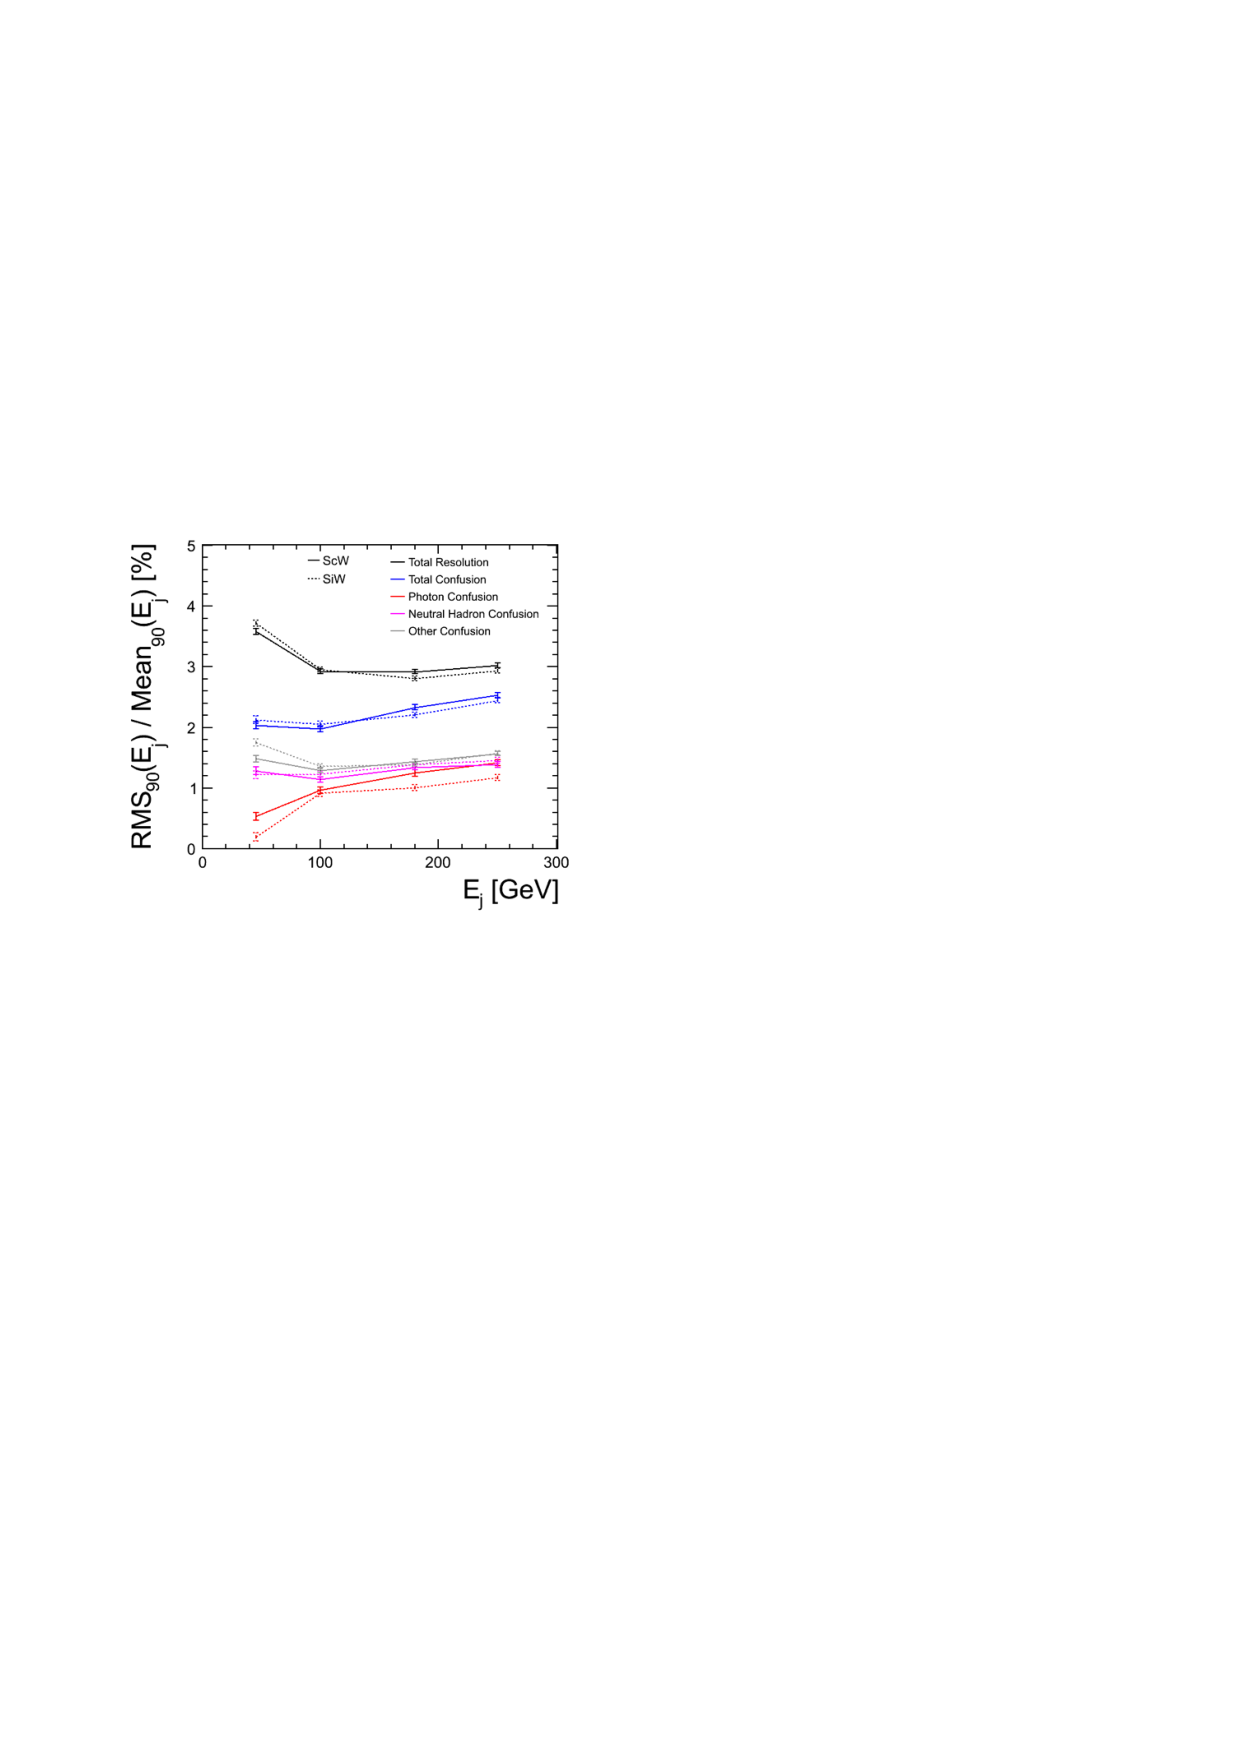
\includegraphics[width=\textwidth]{Software/PandoraPFA/JetEnergyResolution}
		\caption{Jet energy resolution as a function of jet energy, including a breakdown of the
		resolution into contributing ``confusion'' terms. Illustrates performance of
		Pandora algorithms for ILD\_o1\_v06 with Silicon (Si) or Scintillator (Sc) as ECAL
		active material.}
		\label{fig:Software:PandoraPFA:JetEnergyResolution}
	\end{minipage}\hfill
	\begin{minipage}{.49\textwidth}
		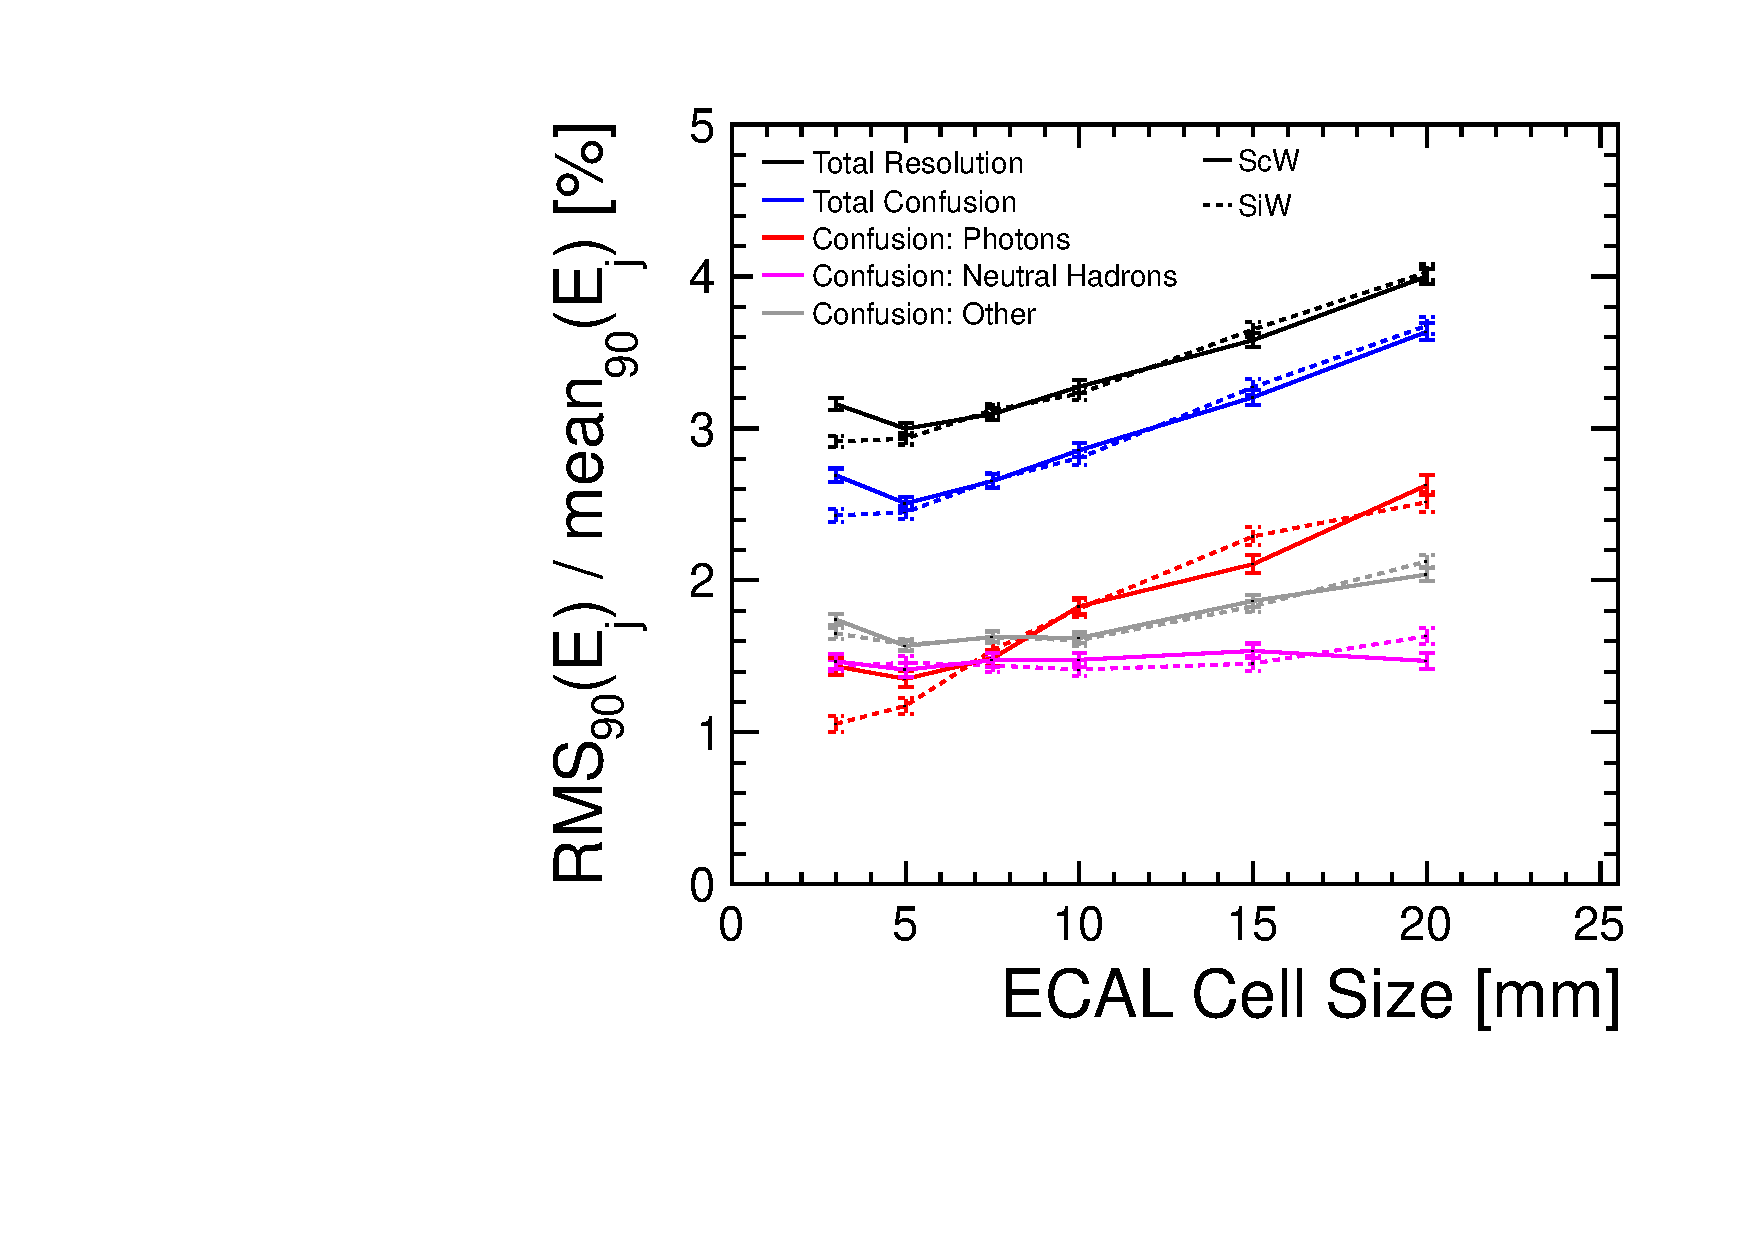
\includegraphics[width=\textwidth]{Software/PandoraPFA/ECAL_CellSize}
		\caption{Jet energy resolution as a function of the ECAL cell size, for \unit[250]{GeV} jets in
		ILD\_o1\_v06. As expected, the photon confusion term (ability to separate photons
		from nearby hadrons) drives performance changes.}
		\label{fig:Software:PandoraPFA:ECAL_CellSize}
	\end{minipage}
\end{figure}

\begin{figure}
\includegraphics[width=.5\textwidth]{Software/PandoraPFA/HCAL_Layers}
\caption{Jet energy resolution as a function of the number of layers in the HCAL, for a range of different energy jets in ILD\_o1\_v06.}
\label{fig:Software:PandoraPFA:HCalLayers}
\end{figure}
